\chapter{TOMAS matching algorithm}
\section{F. Fasseur's work}
F. Fasseur took the idea of the matching algorithm developed for TEXTOR\cite{DesignICRH} and applied it on TOMAS, here I'll quickly discuss the main pointers:
Wirst he did an analysis to the matchable domain from which he found a curve telling us,
given a certain frequency $f$ in the domain [20MHz:48MHz] which $C_a$ value should make the system matchable: 
\begin{figure}[h]
	\centering
	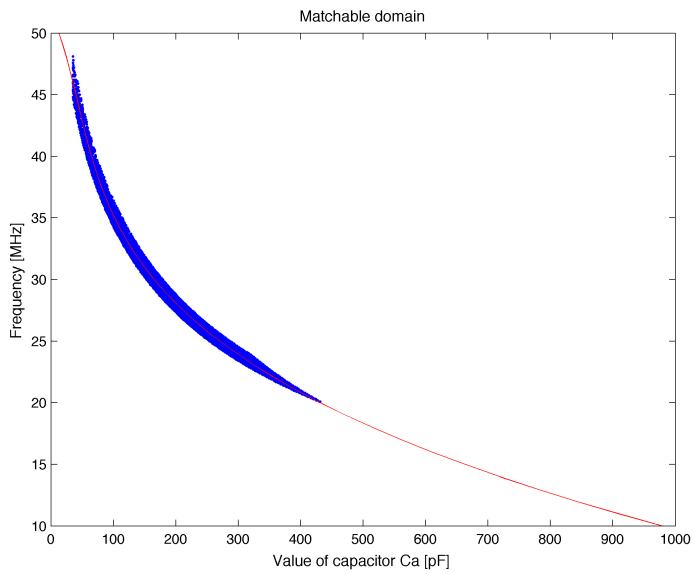
\includegraphics[width=0.5\textwidth]{C_aMatchable}
\end{figure}\\
Of which I analysed the inverse to get the relation
\begin{equation}
	C_a = -3.3094\times 10^{-6}f^5 + 5.17212\times 10^{-4} f^4 -5.10998\times 10^{-2}f^3 + 3.5211f^2 -132.074f + 2000.87
	\label{eqn:C_a}
\end{equation}
In the region 20MHz to 45MHz\footnote{it's worth mentioning that lower
frequencies should also be matchable if the power is capped at 3000W but we
won't concern ourselves with the added complexity}.  Note that the capacitance
seems to be related to the amount of steps as (from the capacitor spec page):
\begin{equation}
	Steps = 0.04781 C_a - 3.68067
	\label{eqn:StepsC_a}
\end{equation}
\newpage
He also designed the following error variables:
\begin{equation}
\epsilon_g = sin(2\beta l_2 )(|V_1| - |V_+|) - sin(2\beta l_1 )(|V_2| - |V_+|)
\end{equation}
\begin{equation}
\epsilon_b = cos(2\beta l_2 )(|V_1| - |V_+|) - cos(2\beta l_1 )(|V_2| - |V_+|)
\end{equation}
Whom are similar to the ones used on TEXTOR. Here $V_1$ and $V_2$ are the voltages at distances $l_1$ and $l_2$ in the power line and $V_+$ the measured forward voltage (using a differential
coupler). 
Here $\beta$ is the so called "phase constant", as we're dealing with a coax cable on TOMAS\footnote{arguably not a very bendy one but not a waveguide}, our
cutoff frequency can be said to be 0 (as the wavelength will be order 30m whilst the perimeter is some 30cm) so we simply have
\begin{equation}
	\boxed{\beta = \frac{\omega}{c} = \frac{2\pi f}{c}}
\end{equation}
These error values are each proportional to a different capacitor:
\begin{eqnarray}
	\epsilon_g &\propto C_s\\
	\epsilon_b &\propto C_p
\end{eqnarray}
The algorithm was simulated for $\pm 3$ turns from the matching point.
\section{Improvement}
Fasseur's work assumes three voltmeters: $V_1$, $V_2$ and $V_+$. 
These only measure amplitude in his setup. in his work he linearizes the equations, 
this was needed in times of TEXTOR (when computations needed to be done using OpAmps) but 
a quick calculation shows that this isn't needed anymore when dealing with the TOMAS setup which has 4 voltmeters. 
The voltage along the line has the form (from transmission line theory):
\begin{equation}
	V_i = V_0^+(e^{i\beta l_i} + \Gamma_L e^{i\beta l_i})
\end{equation}
with $\Gamma_L= u + iv$ the reflection coefficient of the load (the antenna).
from this we can derive that
\begin{equation}
	\frac{|V_i|^2}{|V^+|^2} = 1 + u^2 + v^2 + 2u \cos(2\beta l_i)  + 2v \sin(2\beta l_i) 
\end{equation}
Now, using the absolute voltage measurements we can construct a system of linear equations:
\begin{eqnarray*}
	 u^2 + v^2 + 2u \cos(2\beta l_1)  + 2v \sin(2\beta l_1) &= \frac{|V_1|^2}{|V^+|^2} -1\\
	 u^2 + v^2 + 2u \cos(2\beta l_2)  + 2v \sin(2\beta l_2) &= \frac{|V_2|^2}{|V^+|^2} -1\\
	 u^2 + v^2 + 2u \cos(2\beta l_3)  + 2v \sin(2\beta l_3) &= \frac{|V_3|^2}{|V^+|^2} -1\\
\end{eqnarray*}
Writing this into a matrix:
\begin{equation*}
	\begin{bmatrix}
		1 & 1 & 2\cos(2\beta l_1) & 2\sin(2\beta l_1) & \frac{|V_1|^2}{|V^+|^2} -1\\
		1 & 1 & 2\cos(2\beta l_2) & 2\sin(2\beta l_2) & \frac{|V_2|^2}{|V^+|^2} -1\\
		1 & 1 & 2\cos(2\beta l_3) & 2\sin(2\beta l_3) & \frac{|V_3|^2}{|V^+|^2} -1
	\end{bmatrix}
\end{equation*}
Defining 
\begin{equation}
\boxed{C_i := \cos(2\beta l_i)} \quad \boxed{S_i := \sin(2\beta l_i)} 
\end{equation}
And
\begin{equation}
	\boxed{\frac{|V_i|^2}{|V^+|^2} -1 =: \mathcal{V}_i}
\end{equation}
to help write everything clearer we now have
\begin{equation*}
	\begin{bmatrix}
		1 & 1 & 2C_1 & 2S_1 & \mathcal{V}_1\\
		1 & 1 & 2C_2 & 2S_2 & \mathcal{V}_2\\
		1 & 1 & 2C_3 & 2S_3 & \mathcal{V}_3
	\end{bmatrix}
\end{equation*}
Which gives (substracting the $u^2 + v^2$ terms)
\begin{equation*}
	\begin{bmatrix}
		2(C_1 - C_2) & 2(S_1 - S_2) & (\mathcal{V}_1 - \mathcal{V}_2)\\
		2(C_3 - C_2) & 2(S_3 - S_2) & (\mathcal{V}_3 - \mathcal{V}_2)
	\end{bmatrix}
\end{equation*}
solving for $u$ gives:
\begin{equation}
	\boxed{u = \frac{1}{2}\frac{(\mathcal{V}_1 - \mathcal{V}_2) - (\mathcal{V}_3 - \mathcal{V}_2)\left( \frac{S_1 - S_2}{S_3 - S_2}  \right)}{(C_1 - C_2) - (C_3 - C_2)\left( \frac{S_1 - S_2}{S_3 - S_2}  \right)}}
\end{equation}
and for $v$:
\begin{equation}
	\boxed{v = \frac{1}{2}\frac{(\mathcal{V}_1 - \mathcal{V}_2) - (\mathcal{V}_3 - \mathcal{V}_2)\left( \frac{C_1 - C_2}{C_3 - C_2}  \right)}{(S_1 - S_2) - (S_3 - S_2)\left( \frac{C_1 - C_2}{C_3 - C_2}  \right)}}
\end{equation}
All values shown here are measurable, making it possible to find both $u$ and $v$, so from now on we'll use the variables u and v as if
we have measured them.\\

Matching occurs when $\Gamma_L= 0$ and, as the admittance is given by
\begin{equation}
	y = \frac{1 - \Gamma}{1 + \Gamma} = \frac{1 - u^2 - v^2}{(1+u)^2 + v^2} - i\frac{2v}{(1+u)^2 + v^2} := g + ib
\end{equation}
Matching occurs when $\Re\{y\} := g = 1$ and $\Im\{y\} := b = 0$. So, to probe how close we are to matching, as a first error value we can take b:
\begin{equation}
	\boxed{\epsilon_b = -\frac{2v}{(1+u)^2 + v^2}}
\end{equation}
and as a second error we'll take $1-g$:
\begin{equation}
	\boxed{\epsilon_g = 1 - \frac{1 - u^2 - v^2}{(1+u)^2 + v^2}}
\end{equation}
So finally, as we know both u and v, to match the system the change in capacitance will have to vary as:
\begin{eqnarray}
	\Delta C_s \propto \epsilon_g\\
	\Delta C_p \propto \epsilon_b
\end{eqnarray}
As both variable capacitors are linear, we can say that the amount of steps required can be gives by
\begin{eqnarray}
	\Delta C_s := S\epsilon_g\\
	\Delta C_p := P\epsilon_b
\end{eqnarray}
With $S$ and $P$ constants we may determine from running a simulation or by doing experiments.
\section{Practical implementation}
Applying the algorithm would thus look as follows:
\begin{enumerate}
	\item use equations \ref{eqn:C_a} and \ref{eqn:StepsC_a} to move the prematching capacitor according to the selected frequency.
	\item lower the power to 1000W as to not damage any components whilst tuning and start the ICRH antenna
	\item Record the various needed measurements over some sufficiently big time $\Delta t$ (to reduce noise) and send them over from matlab to the python gui 
	\item Compute the various errors, stop the algorithm if either 
		\begin{itemize}
			\item $\epsilon_b < \Delta_b$ and $\epsilon_g < \Delta_g$ 
			\item $\Gamma_L <$ some percentage
		\end{itemize}
	\item As the response of both the parallel and series capacitor are linear, compute the steps using Steps C_s $\propto\epsilon_g$ and Steps C_p$\propto\epsilon_b$
	\item adjust the capacitors
	\item back to 3.
\end{enumerate}
\begin{figure}[h]
	\centering
	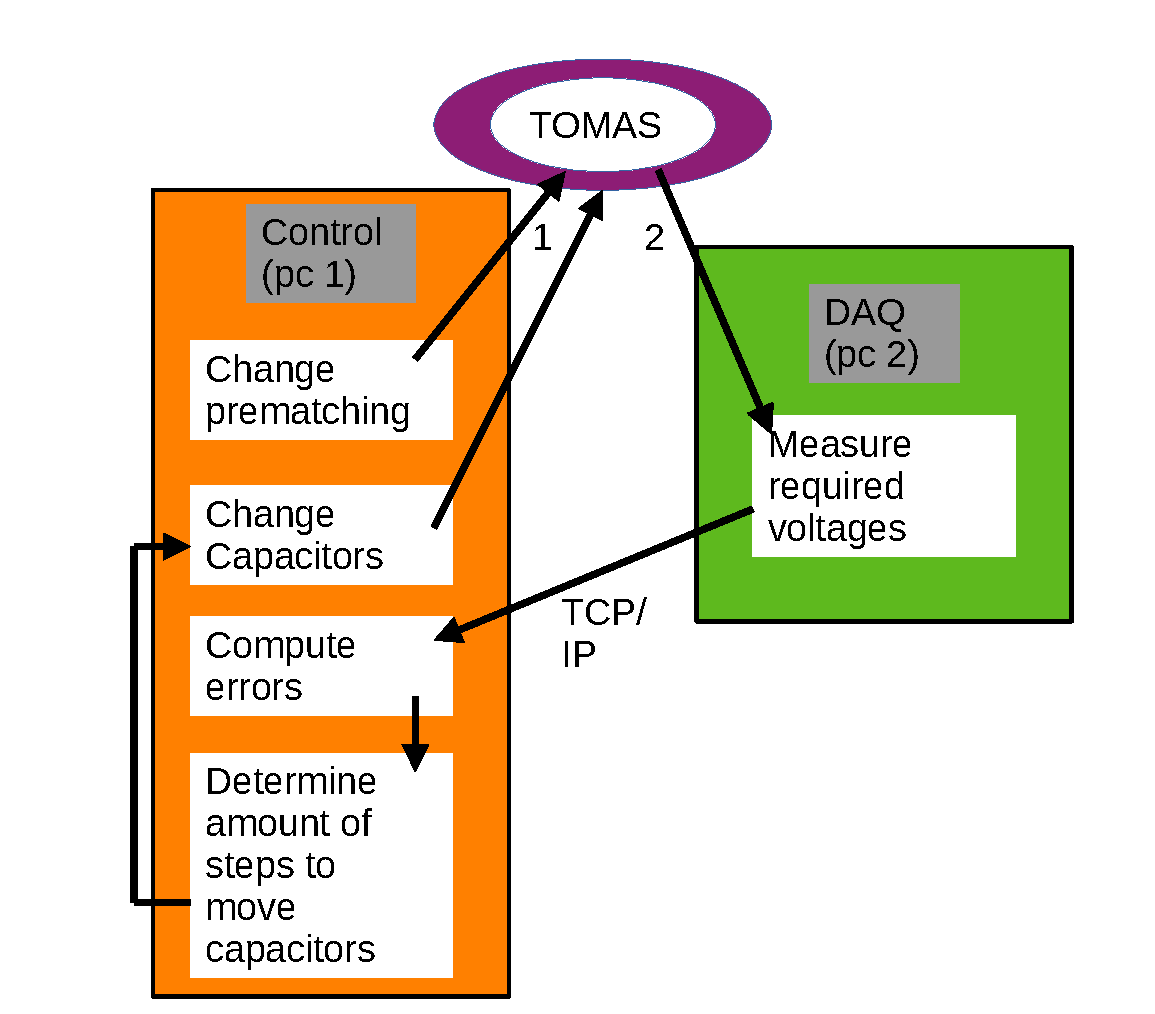
\includegraphics[width=0.4\textwidth]{MatchingSystem.pdf}
	\caption{Overview of the system, pc2 will communicate it's data with pc1 through TCP/IP whilst pc1 is triggered using a biasing voltage from pc2}
	\label{fig:system}
\end{figure}
After sufficient loops, the errors will fluctuate less than the predefined values $\Delta_g$ and $\Delta_b$ or the reflection coeffeciënt is sufficiently small and the matching algorithm may stop.

